\subsection{Tumour derived network to stratify MIBC} \label{s:N_I:tum}


The Parsimonious Gene Correlation Analysis Network Analysis (PGCNA) was used to stratify breast, colon, and glioblastoma cancers \cite{Care2019-ij,Tanner2023-wa} based on gene expression. With the goal to better inform the MIBC subtyping, in this section we developed an integrative network approach to stratify MIBC. Our model differs from PGCNA by building the network using both gene expression and mutation as well as  domain knowledge through Transcription Factors (TFs).

\subsubsection{Describing the network} \label{s:N_I:tum_describe}

The network weights are modified to integrated the mutation burden across the TCGA cohort into the network. The changes are applied after the Spearman correlation matrix is computed but before the edge pruning. The reward strategy '\textit{promotes}' the genes which are highly mutated across tumours by increasing their weight, conversely the penalised strategy \textit{punishes} the genes that are highly mutated. The two modifiers are described in Figure \ref{fig:N_I:modifiers} where the highest mutated genes (e.g. TP53, TTN) are the most penalised/rewarded, while the weight values for un-mutated genes remain unchanged. It is worth mentioning, that there is no need to adapt the ModCon as the weight changes will affect the connectivity parameters from Equation \ref{eq:modcon}.

\begin{figure}[!htb]    \centering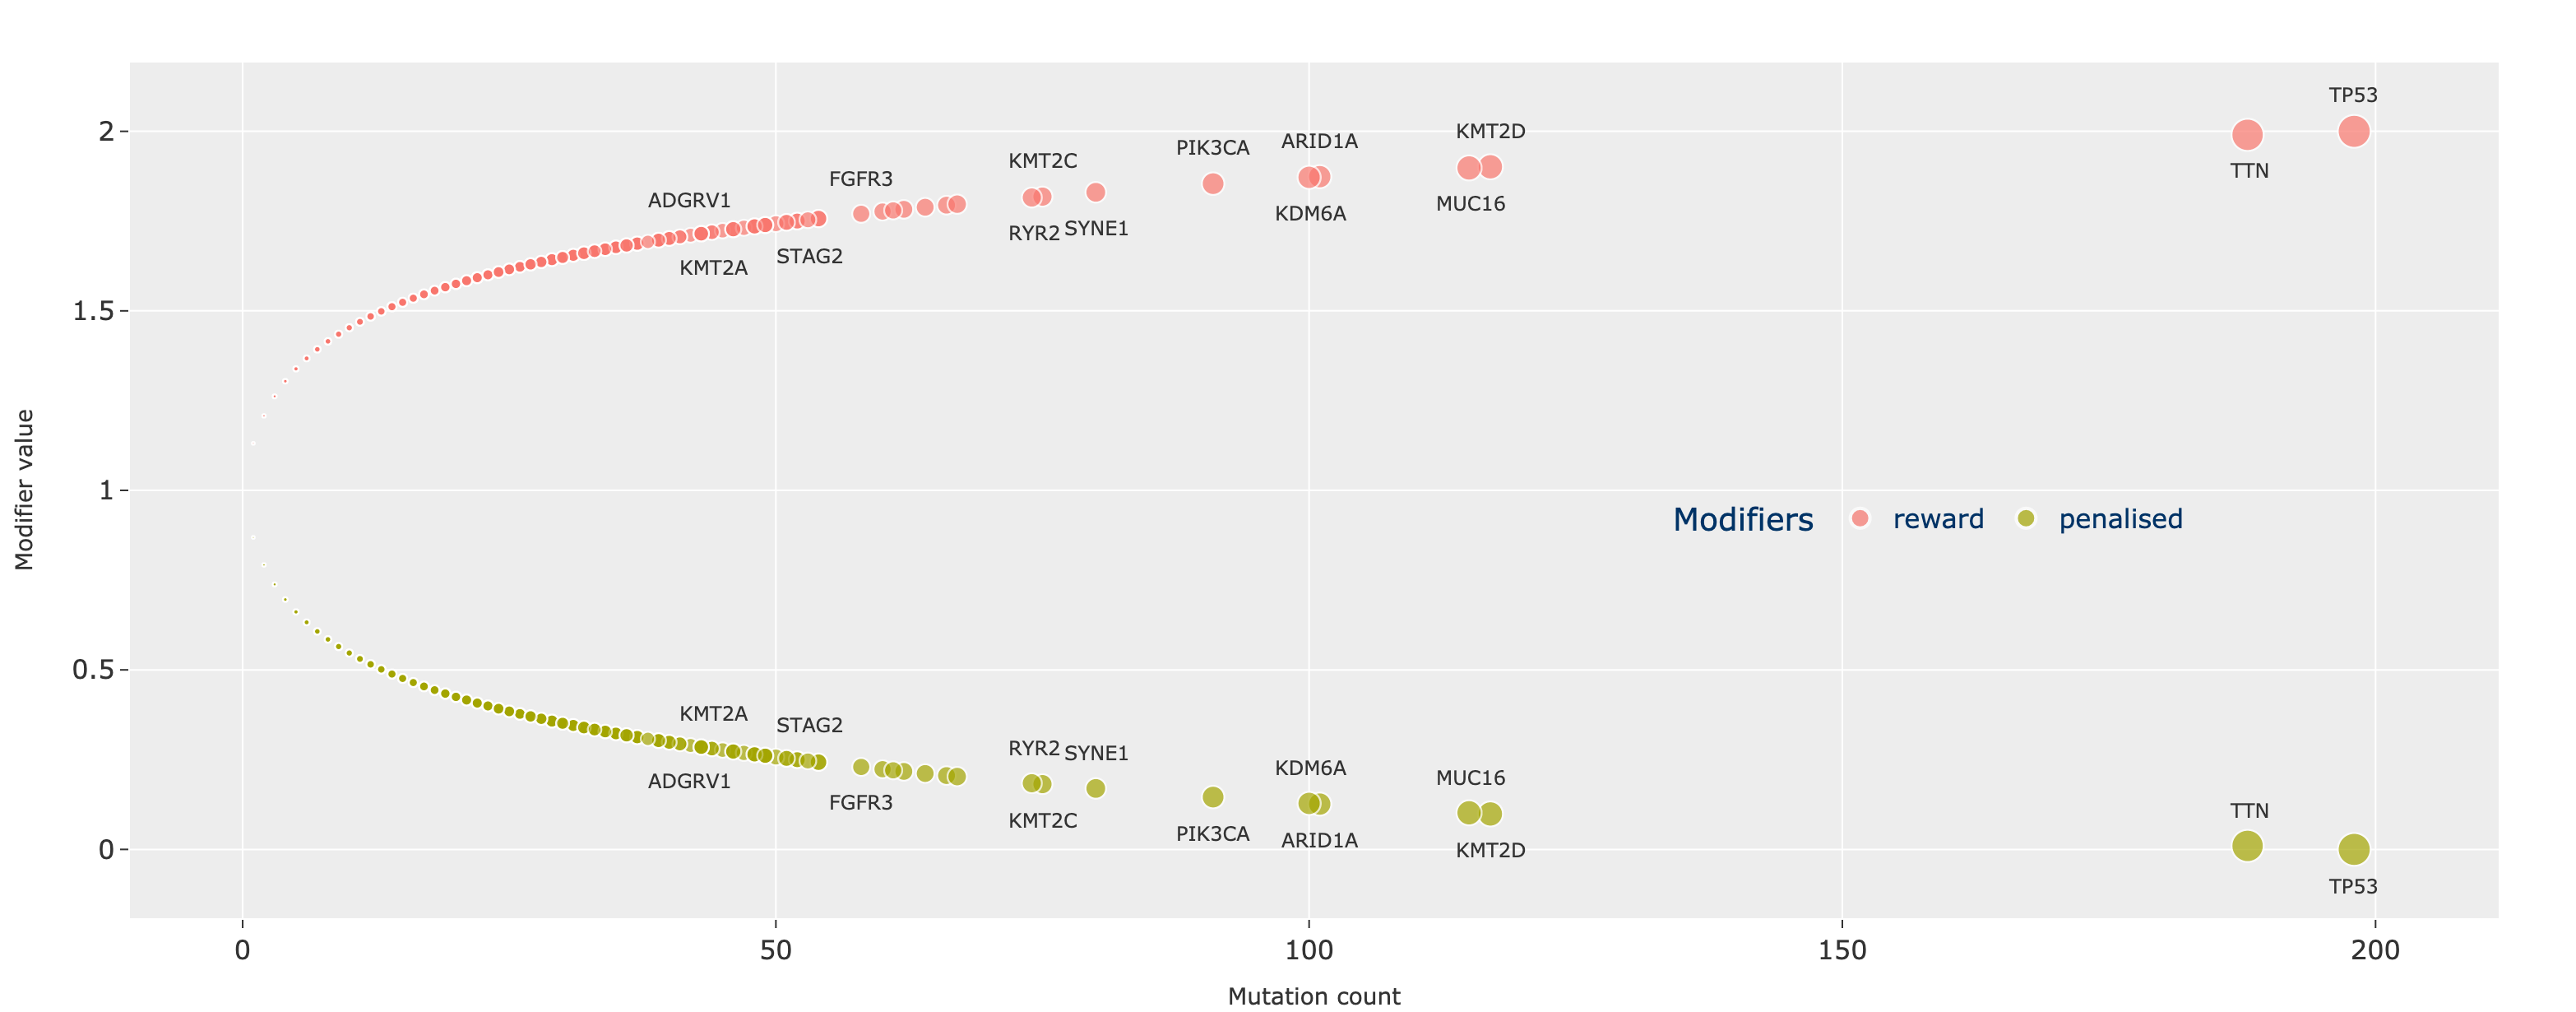
\includegraphics[width=0.9\textwidth,height=0.9\textheight,keepaspectratio]{Sections/Network_I/Resources/Methods/modifiers.png}
    \caption{Representing the two weight modifier strategies employed at the network construction stage. The blue, reward strategy, awards the genes that have a high burden across the cohort. Conversely, the  penalised strategy decreases the edges' strength for highly mutated genes. In both cases, the un-mutated genes remain unchanged.}
    \label{fig:N_I:modifiers}
\end{figure}


The node degree represents the number of connections a node has, a higher number, the more important the node is to the network. However, it is not only important how many connections there are but also to which nodes are these linked to for which PageRank\cite{Brin1998-mc} accounts. Thus, degree and PageRank are used in this project to described the network's centrality. It is also important how close the nodes are and if a node is an intermediate between others, thus the closeness and betweeness metrics are employed to describe the network. In addition, the Integrated Value of Influence (IVI) \cite{Salavaty2020-wo} combines multiple metrics and it is used to score the nodes have both a local and global influence to the network.

\begin{figure}[!htb]    \centering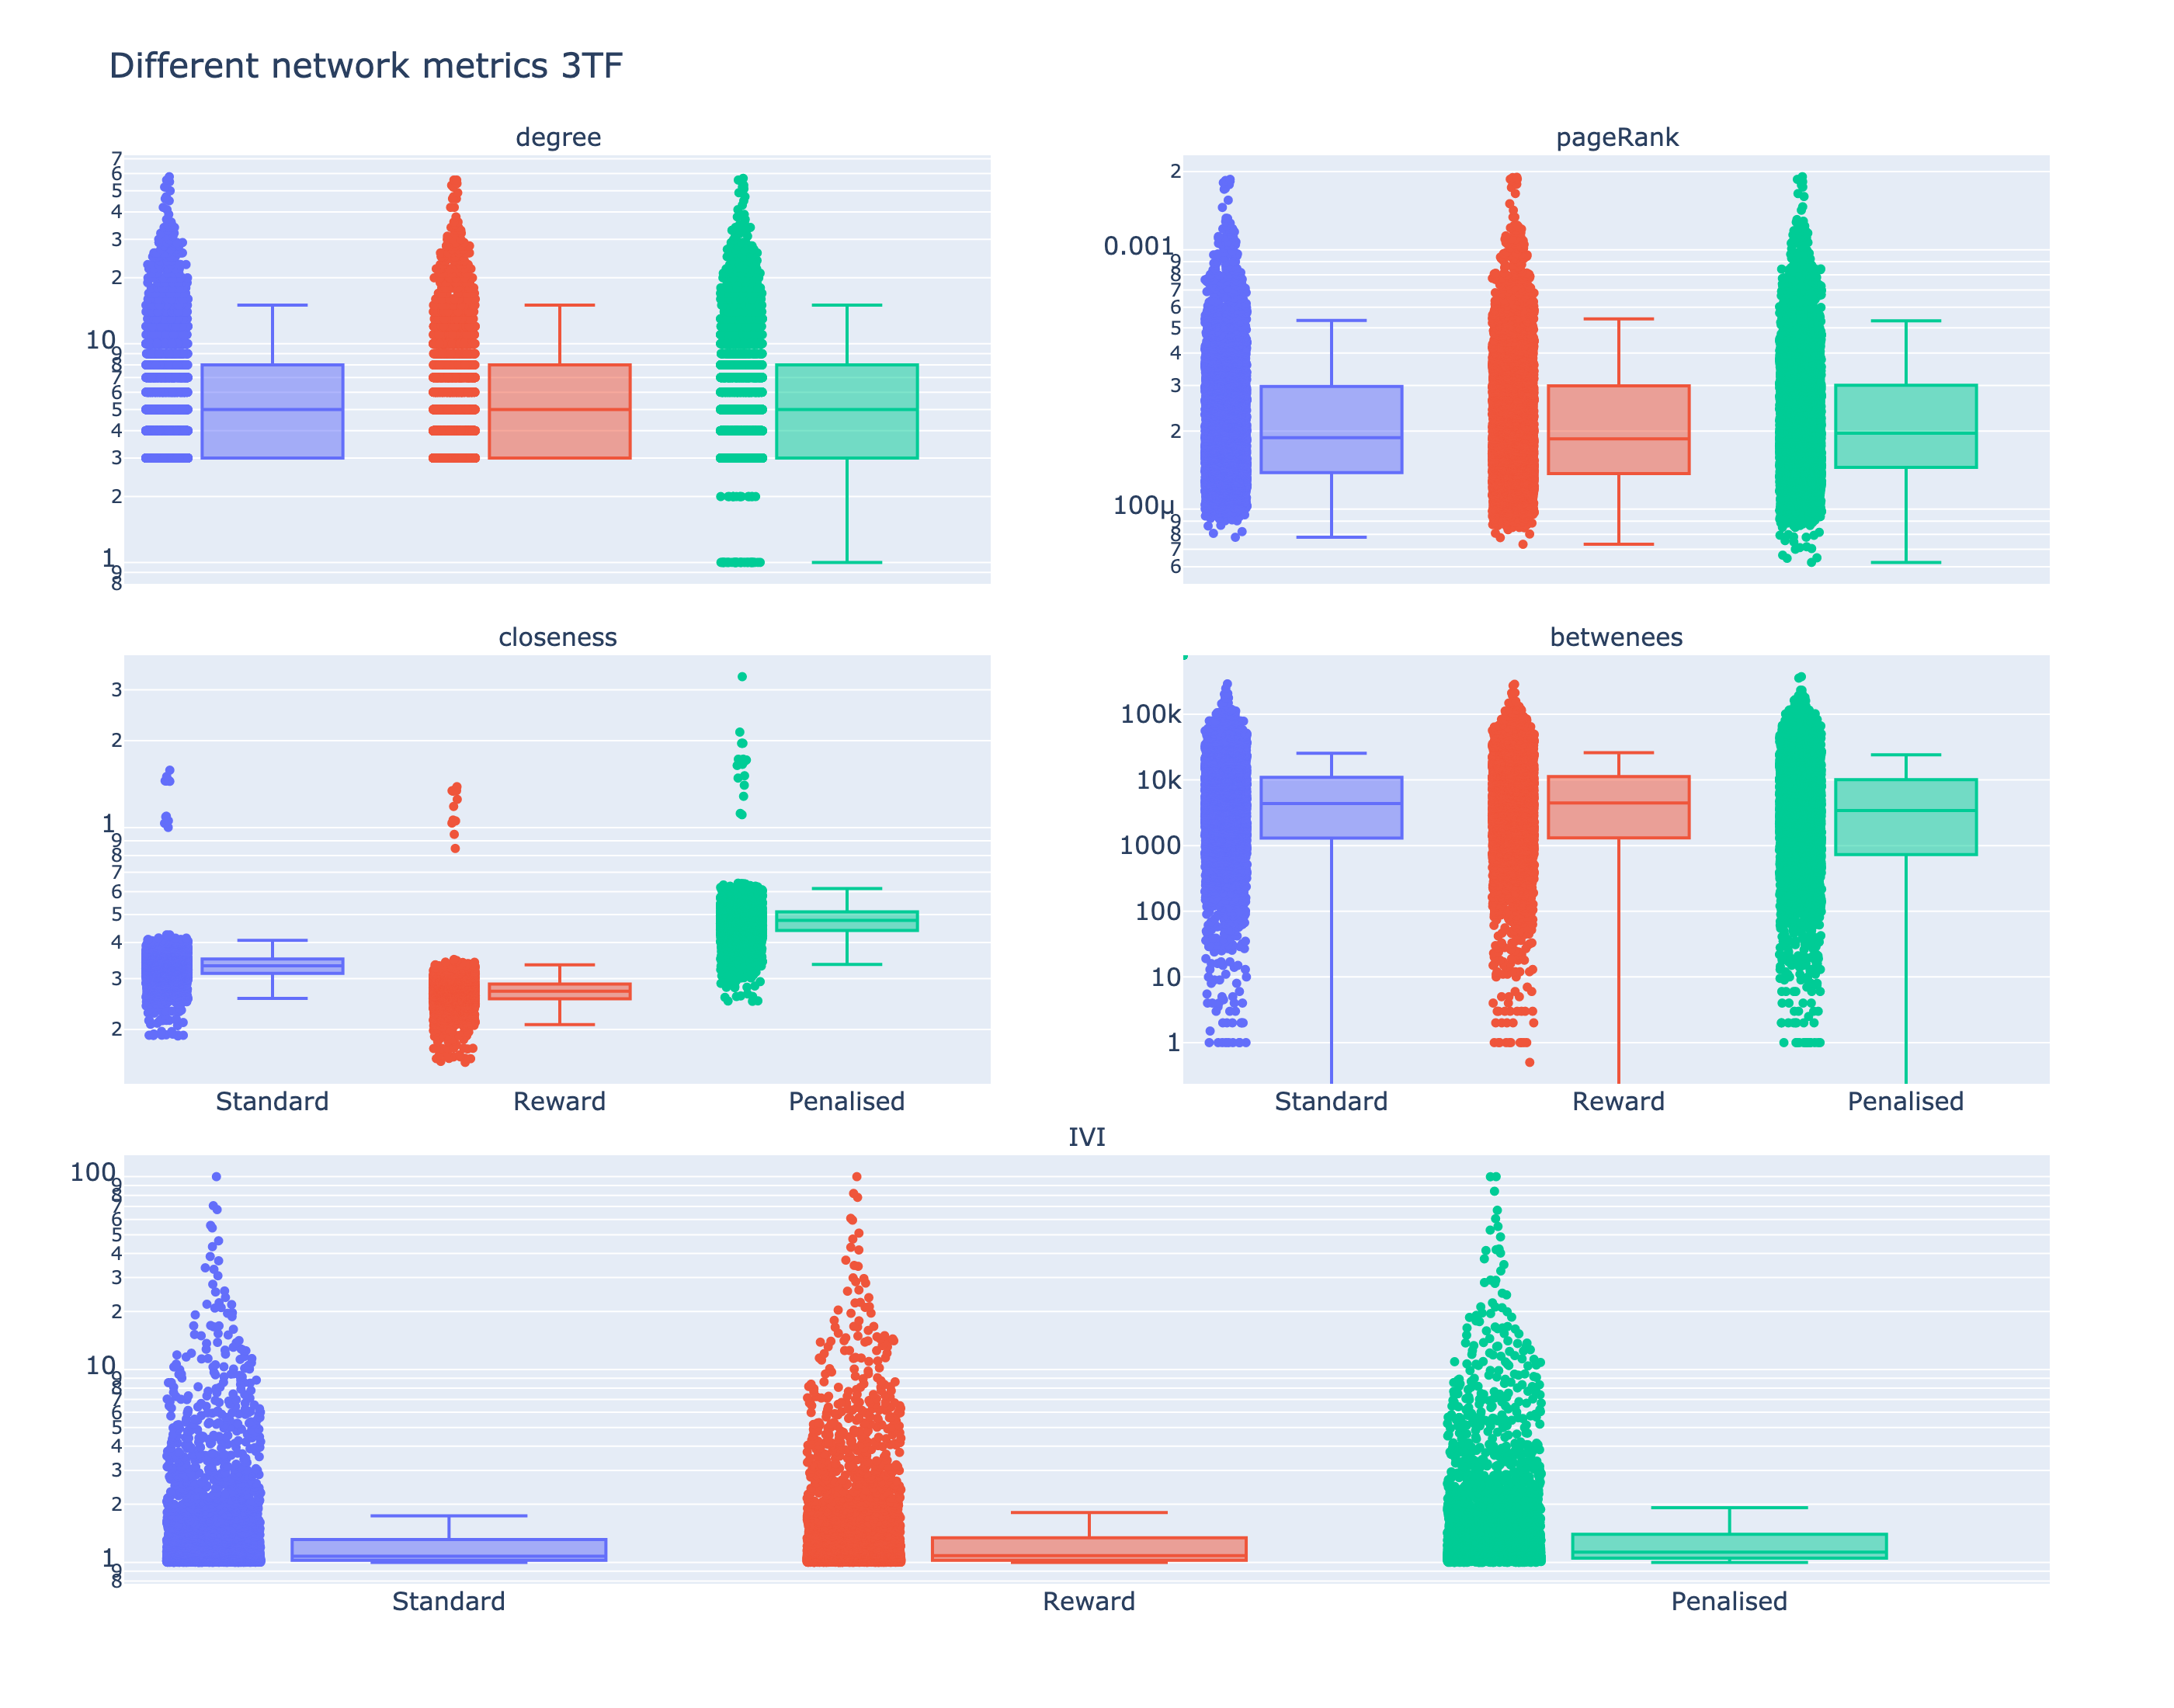
\includegraphics[width=1.0\textwidth,height=0.7\textheight,keepaspectratio]{Sections/Network_I/Resources/Tum_network/NetworkMetricsComp_10TF.png}
    \caption{Network metrics for the tumour networks formed from 4K genes, 3 connections per standard gene and 10 for TFs with the different weight modifiers; standard (blue), reward (red) and penalised (green). The y-axis represent the log10 of the metric. }
    \label{fig:N_I:net_metrics_tum}
\end{figure}

The different network metrics for standard (blue), reward (red) and penalised (green) are shown in Figure \ref{fig:N_I:net_metrics_tum}. The network metrics are generally similar across the different type modifiers with the exception of the penalised network where the nodes' degree is negatively affected and the the nodes are usually closer to each other (higher closeness values). This is due to the penalised function which almost prunes the connections for the highly mutated genes.

\begin{figure}[!htb]    \centering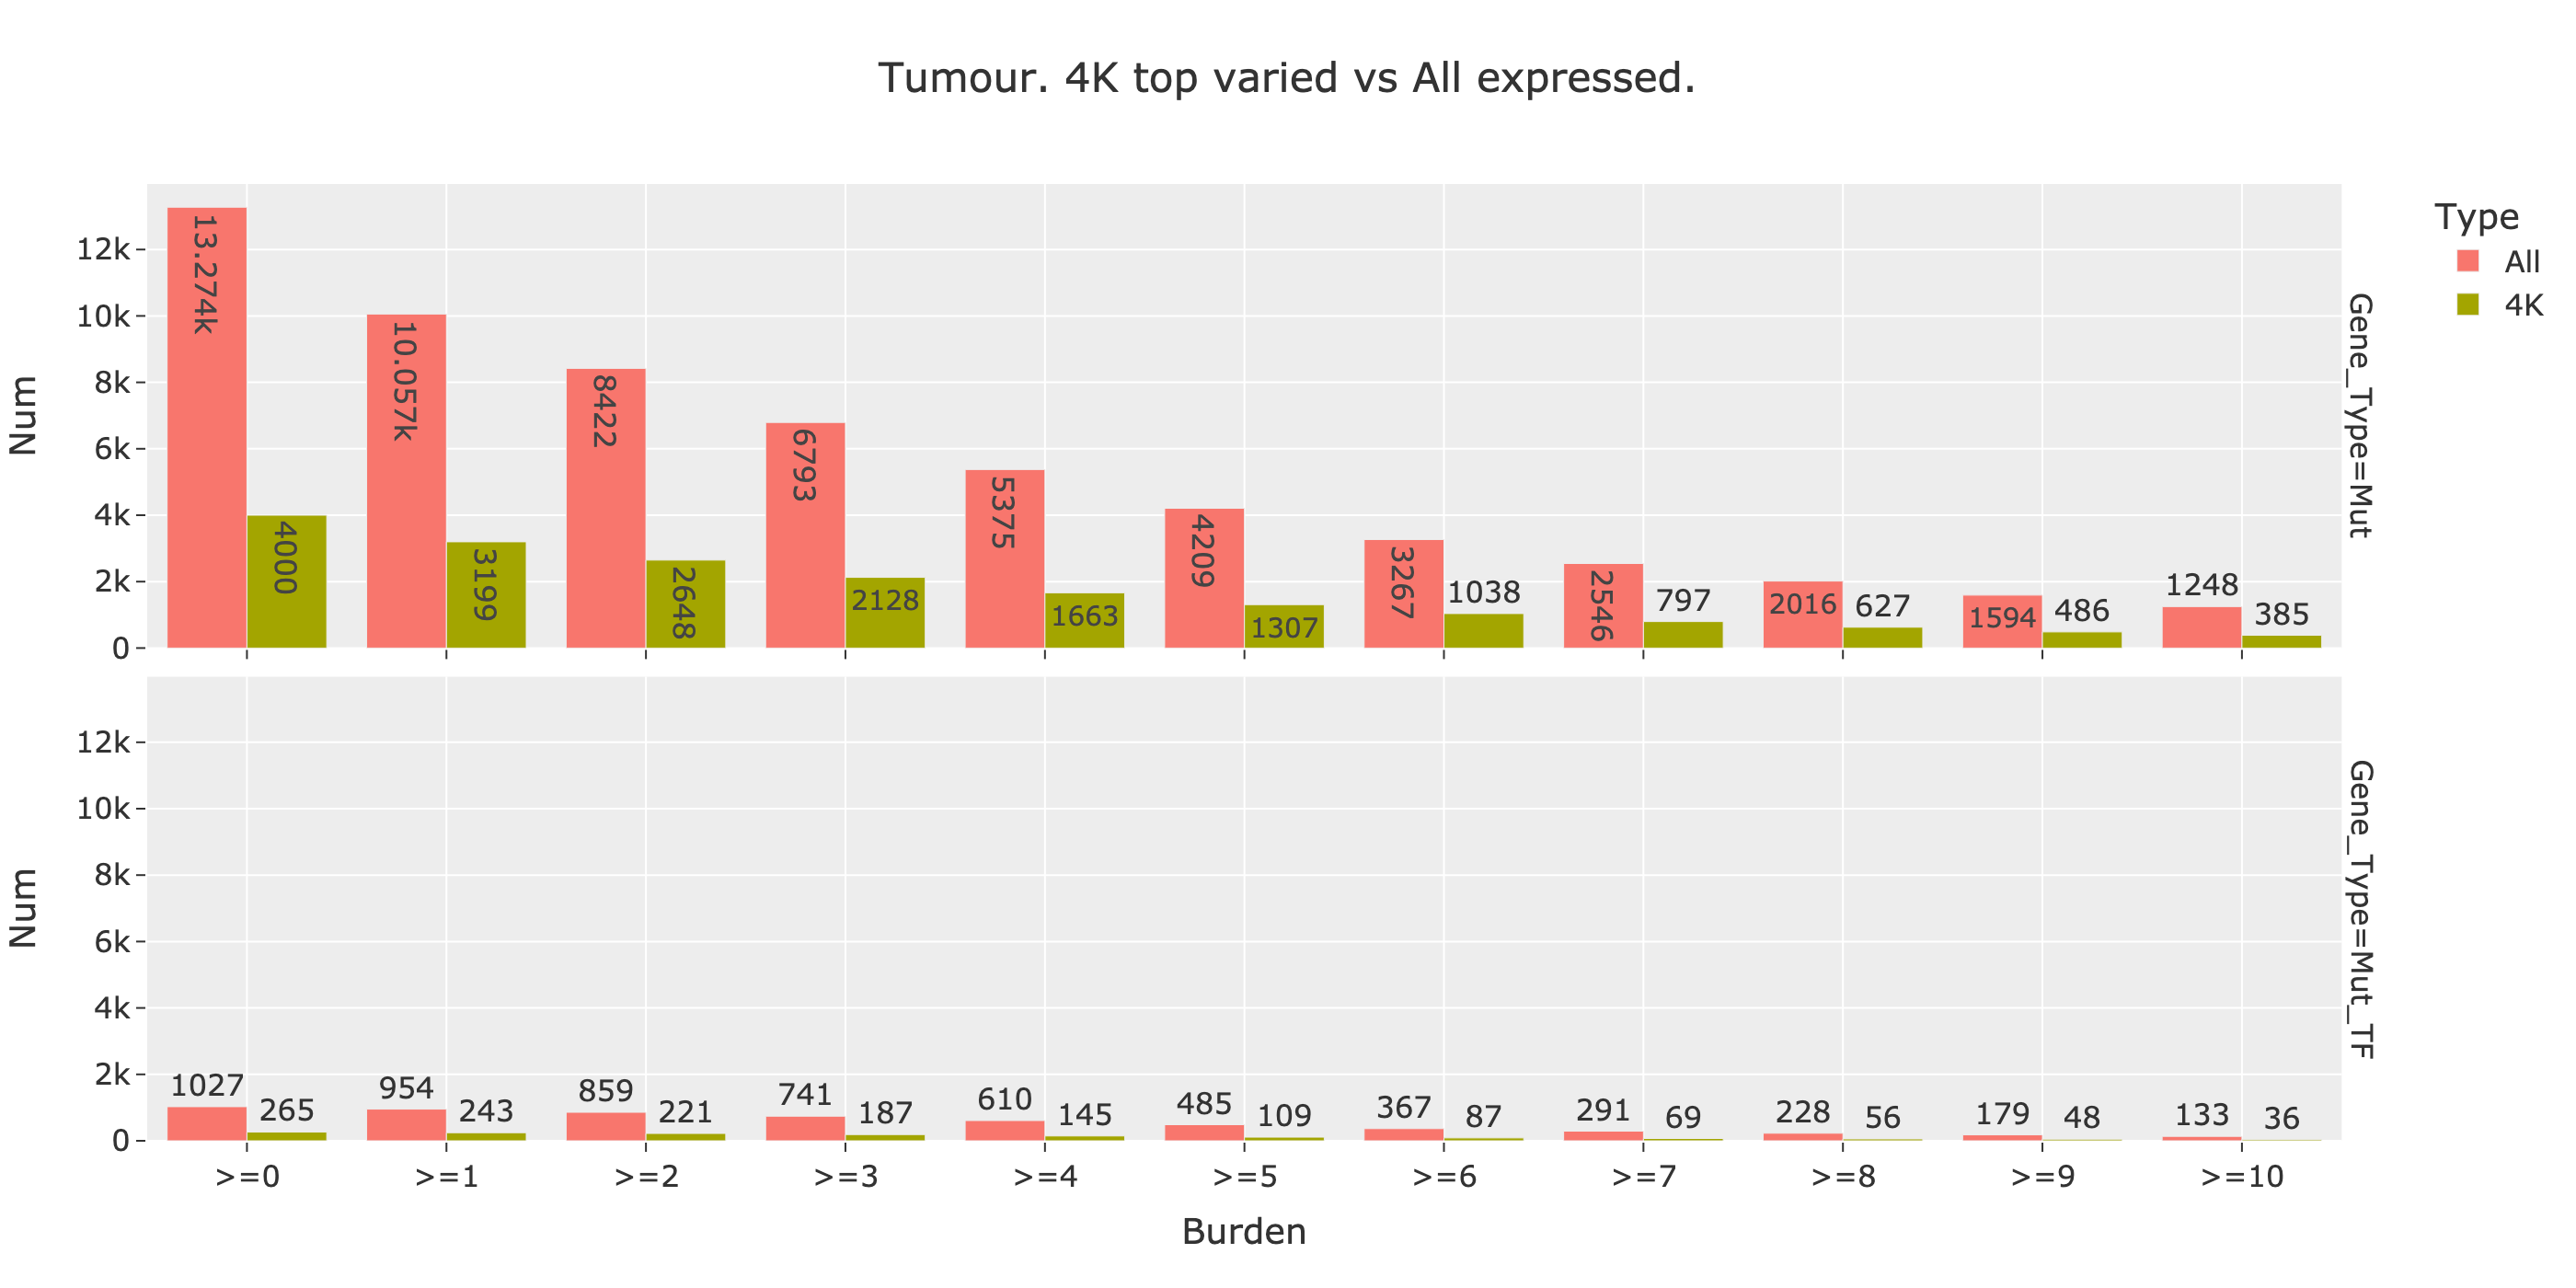
\includegraphics[width=1.0\textwidth,height=0.6\textheight,keepaspectratio]{Sections/Network_I/Resources/Tum_network/MutTF_representation_4K-all.png}
    \caption{Mutation representation in the 4K most varied genes vs all the genes expressed.}
    \label{fig:N_I:mut_rep_tum}
\end{figure}


There are $\approx30K$ genes in the TCGA's MIBC cohort, from which less than a half ($\approx13K$) are considered expressed; more than 3 samples have TPM values larger than 0.5. From the $\approx13K$ genes there are $\approx10K$ genes which are mutated at least once, but then as the mutation count is increased there are less genes represented as seen in Figure \ref{fig:N_I:mut_rep_tum}. The same trend can be noticed for TFs genes initially being 1027 genes in all the expressed genes, but only a few are mutated. The striking aspect of the Figure \ref{fig:N_I:mut_rep_tum} is the \textbf{steep decrease??} of the genes mutated, we have explored different genes selection strategies in Section \ref{}.

\begin{figure}[!htb]    \centering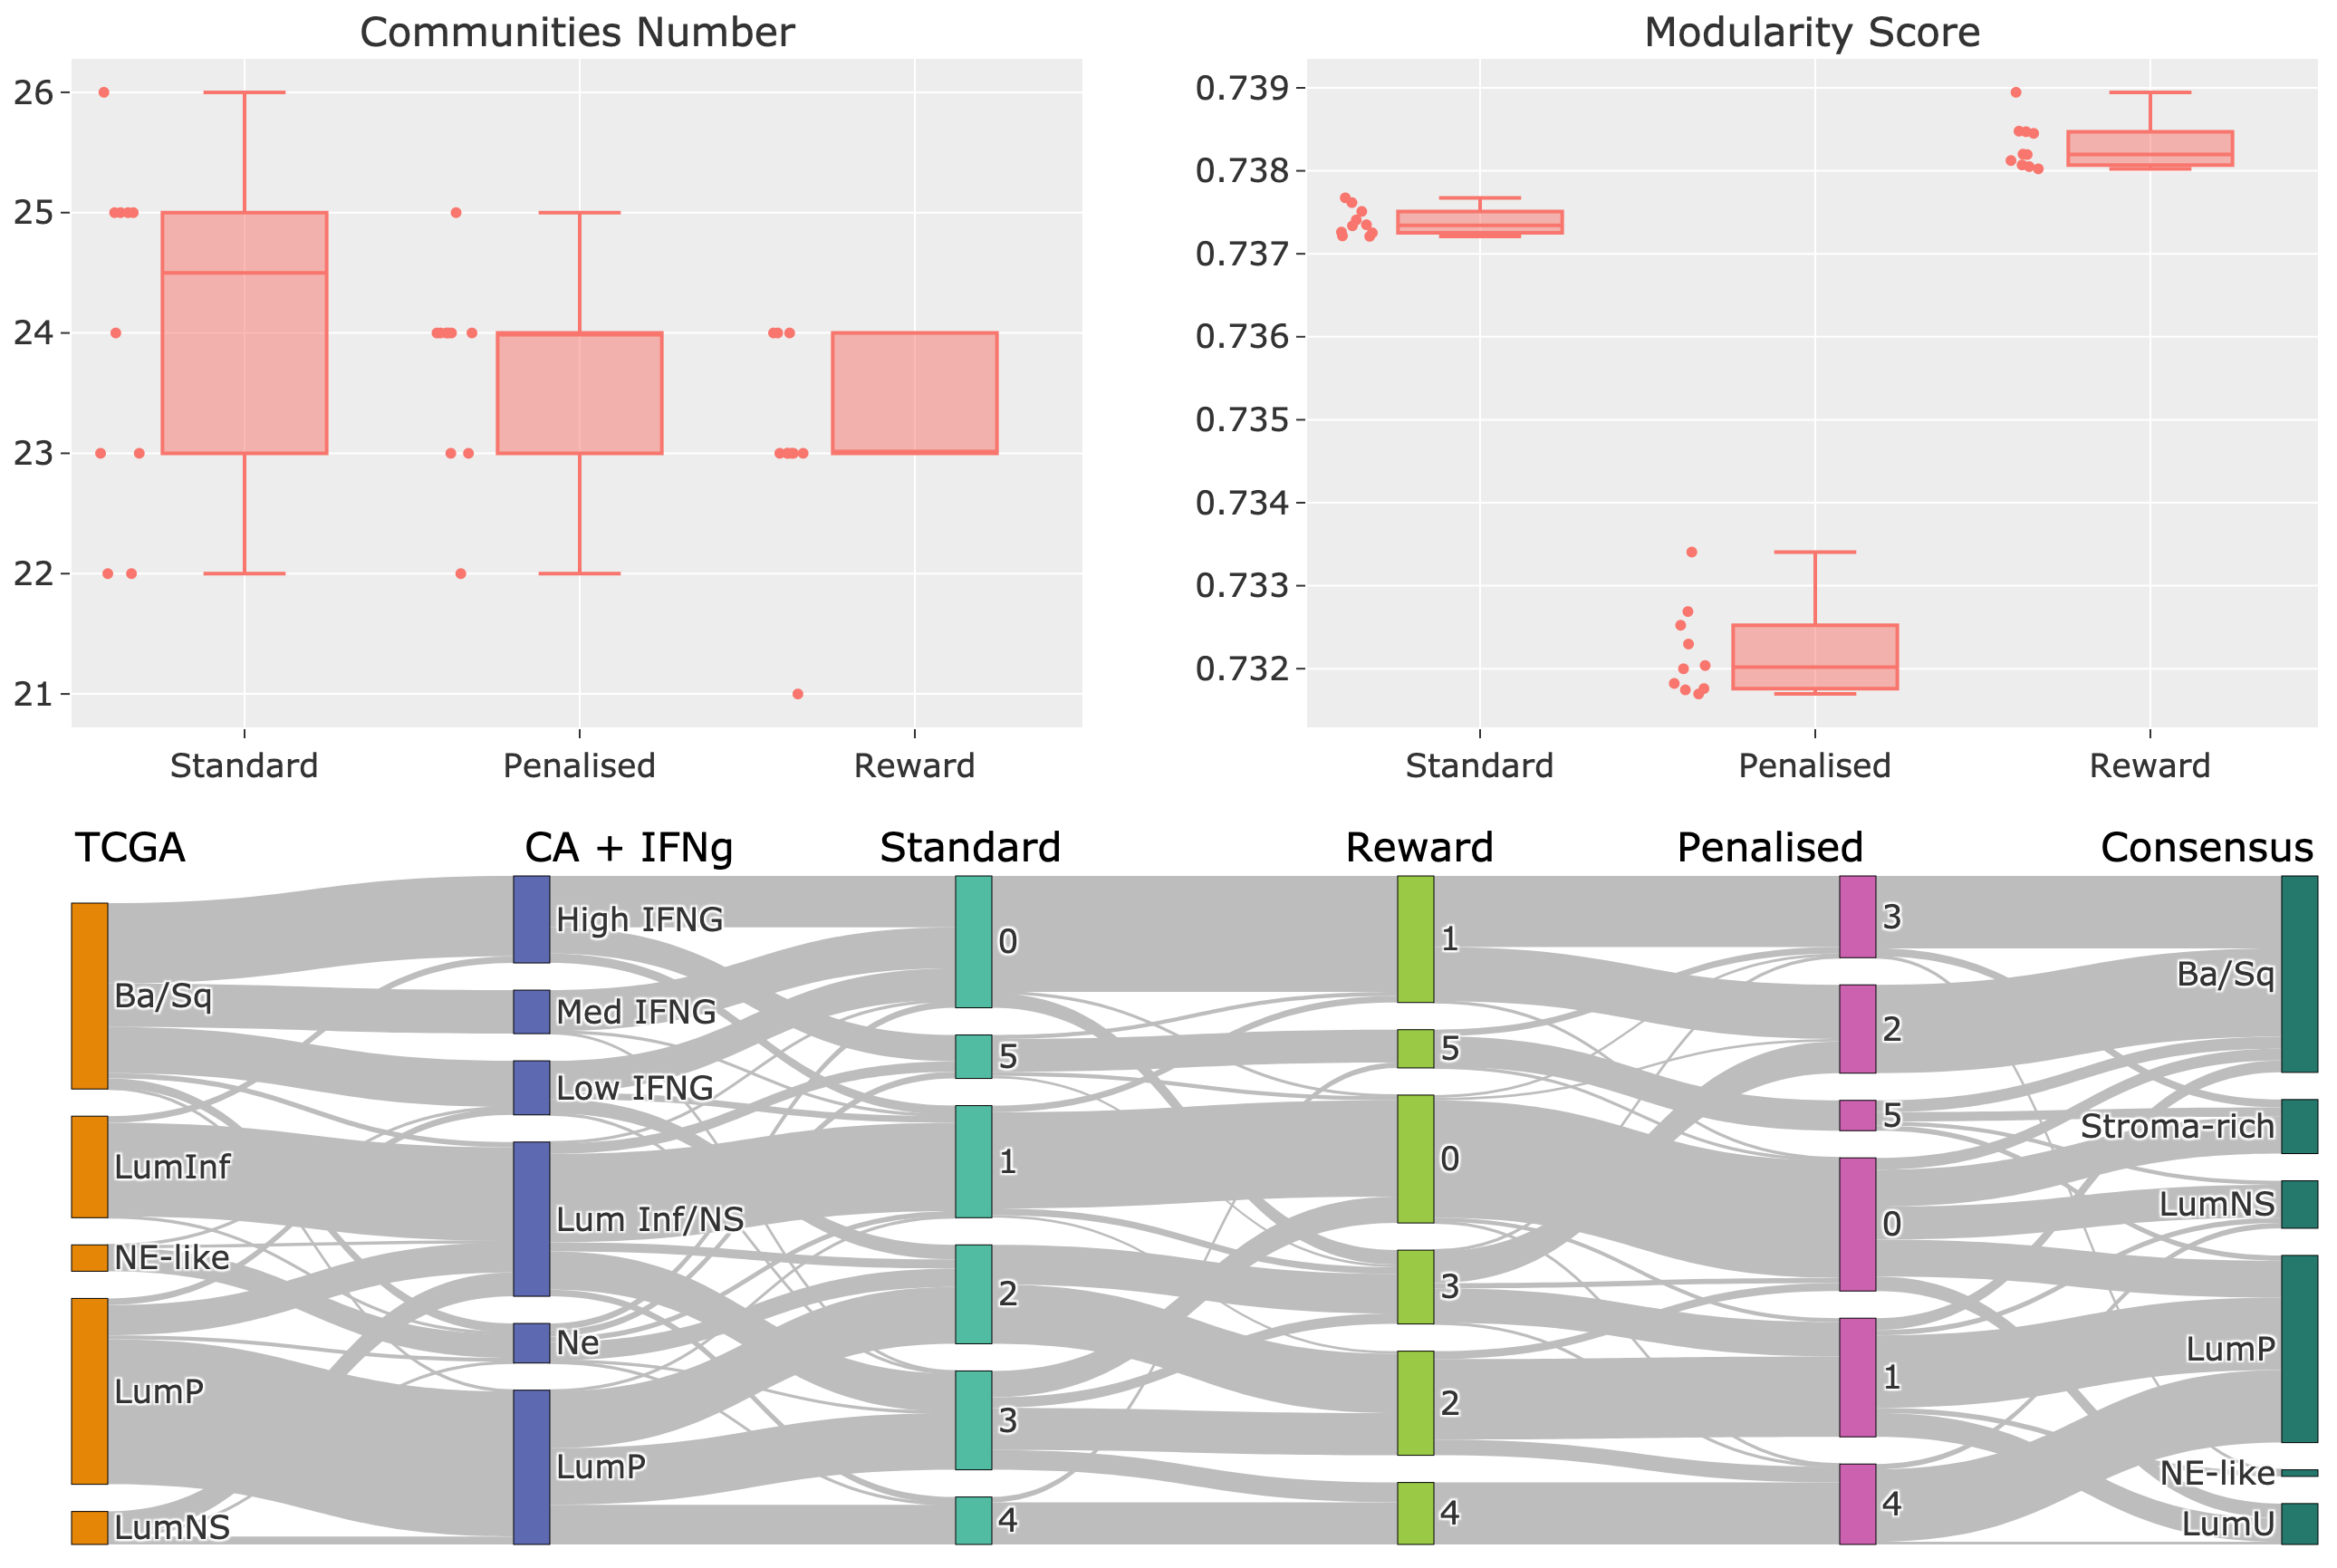
\includegraphics[width=1.0\textwidth,height=0.6\textheight,keepaspectratio]{Sections/Network_I/Resources/Tum_network/LeidenMetrics_Sankey_TF-6.png}
    \caption{On the top are displayed the community size and Modularity Score. The two metrics used to asses the weight modifiers (Standard, Penalty and Reward) the Leiden algorithm. At the bottom the Sankey plot to show the MIBC subtyping using the different standard classifiers (TCGA and consensus) with our previous developed clustering and the three different networks. }
    \label{fig:N_I:tum_leiden_modifiers}
\end{figure}

\subsubsection{Community detection and MIBC stratification}

Modularity score is used to measure the community separation and to evaluate performance of the Leiden community detection algorithm. The Standard and Reward have higher Modularity scores compared to the Penalised network as seen in Figure \ref{fig:N_I:tum_leiden_modifiers}. The unmodified network consistently finds more communities than the other 2 modified networks. 


After applying ModCon the important genes from the network we then apply K-means (K=6) clustering on the MEV values to find the MIBC subtypes. As the goal of this set of experiments was to understand the changes in the MIBC subtypes derived from the different weight modifiers. To avoid introducing other variables and to be consistent with our previous findings (see Section \ref{}) where K-means with K=6 (or 5) was found to exhibit the most separated clusters, thus K-means with K=6 on the MEV score. Clustering analysis is performed on MEV scores for the P0 network in Section \ref{s:p0:clustering_analysis} 

At the bottom of Figure \ref{fig:N_I:tum_leiden_modifiers} the Sankey plot shows the differences in the MIBC subtypes between the 3 type of networks, the literature (TCGA \& consensus) and our previous classification. All the networks split into two smaller groups (Reward and Standard - \textbf{3\&1}; Penalised - \textbf{3 \& 2}) the Luminal Papillary (LumP) and Luminal Infiltrated/Non-Specified (LumInf/NS) is consistently clustered in one group (0). However, there are more changes in the Basal split and Ne. The Standard and Reward are consistent in finding the same 3 groups (\textbf{5, 4 and 2}) where\textbf{ 5} is a mixed of LumInf/NS and High IFNg,\textbf{4} is mainly Low IFNG and a few NE samples while \textbf{2} is a combination of High and Medium IFNg. This may suggest that cluster 4 may represent the tumours which are more basal (de-differentiated), while \textbf{5} the tumours with high infiltration and immune response and cluster \textbf{2} the samples between the two. In the Penalised network sub-grouping the cluster \textbf{5} remains the same, but \textbf{4} and \textbf{1} are changed. The former contains more of the LumP and Low IFNG samples, while the latter hold most of the IFNG samples. This suggest that the Penalised network stratification perform worst.

Overall, the stratification shown in Figure \ref{fig:N_I:tum_leiden_modifiers} shows the potential of the Network approach by finding similar three Basal subgroups as in our previous clustering where we used both computational method and domain knowledge from in-vitro study\citet{Baker2022-bj}. However, there is little difference between the networks suggesting that there weight modifiers do not have a high impact on MIBC stratification with K-means (K=6).

\subsubsection{Clustering analysis vs Network gene selection} \label{s:N_I:cs_vs_gene_sel}

Crudely simplified the network approach is an advance gene selection mechanism based on multiple data-types: gene co-expression, mutation and transcription factors. Specifically, the Module Connectivity step from Figure \ref{fig:N_I:network_pipeline} picks the genes that have the highest connectivity (see Eq. \ref{eq:modcon}) and varied across the dataset, which are then used for clustering analysis (through MEV). Similarly, in the previous chapter $\approx3K$ top most relative varied genes were used in the K-means clustering analysis. Therefore, there is a need to compare the two gene selection methods and to assess the differences.

The comparison is performed only using the TCGA's MIBC dataset to avoid differences between the tumour and healthy samples. The network was constructed from the 5K most varied genes, no weight modifier and the minimum degree for TFs  was set to 6 and 3 to the standard genes. For a network formed of 5K genes, the ModCon (=100 for each community) selects in total $\approx2.8K$ genes. The TF configuration to keep 6 edges per TF is selected based on the experiment in Section \ref{}\footnote{Selective edge pruning experiments} where it was observed that more than 10 edges per TF does not influence the network and the 3 connections is the standard, thus we selected the middle value for the gene comparison.


\begin{figure}[!htb]    \centering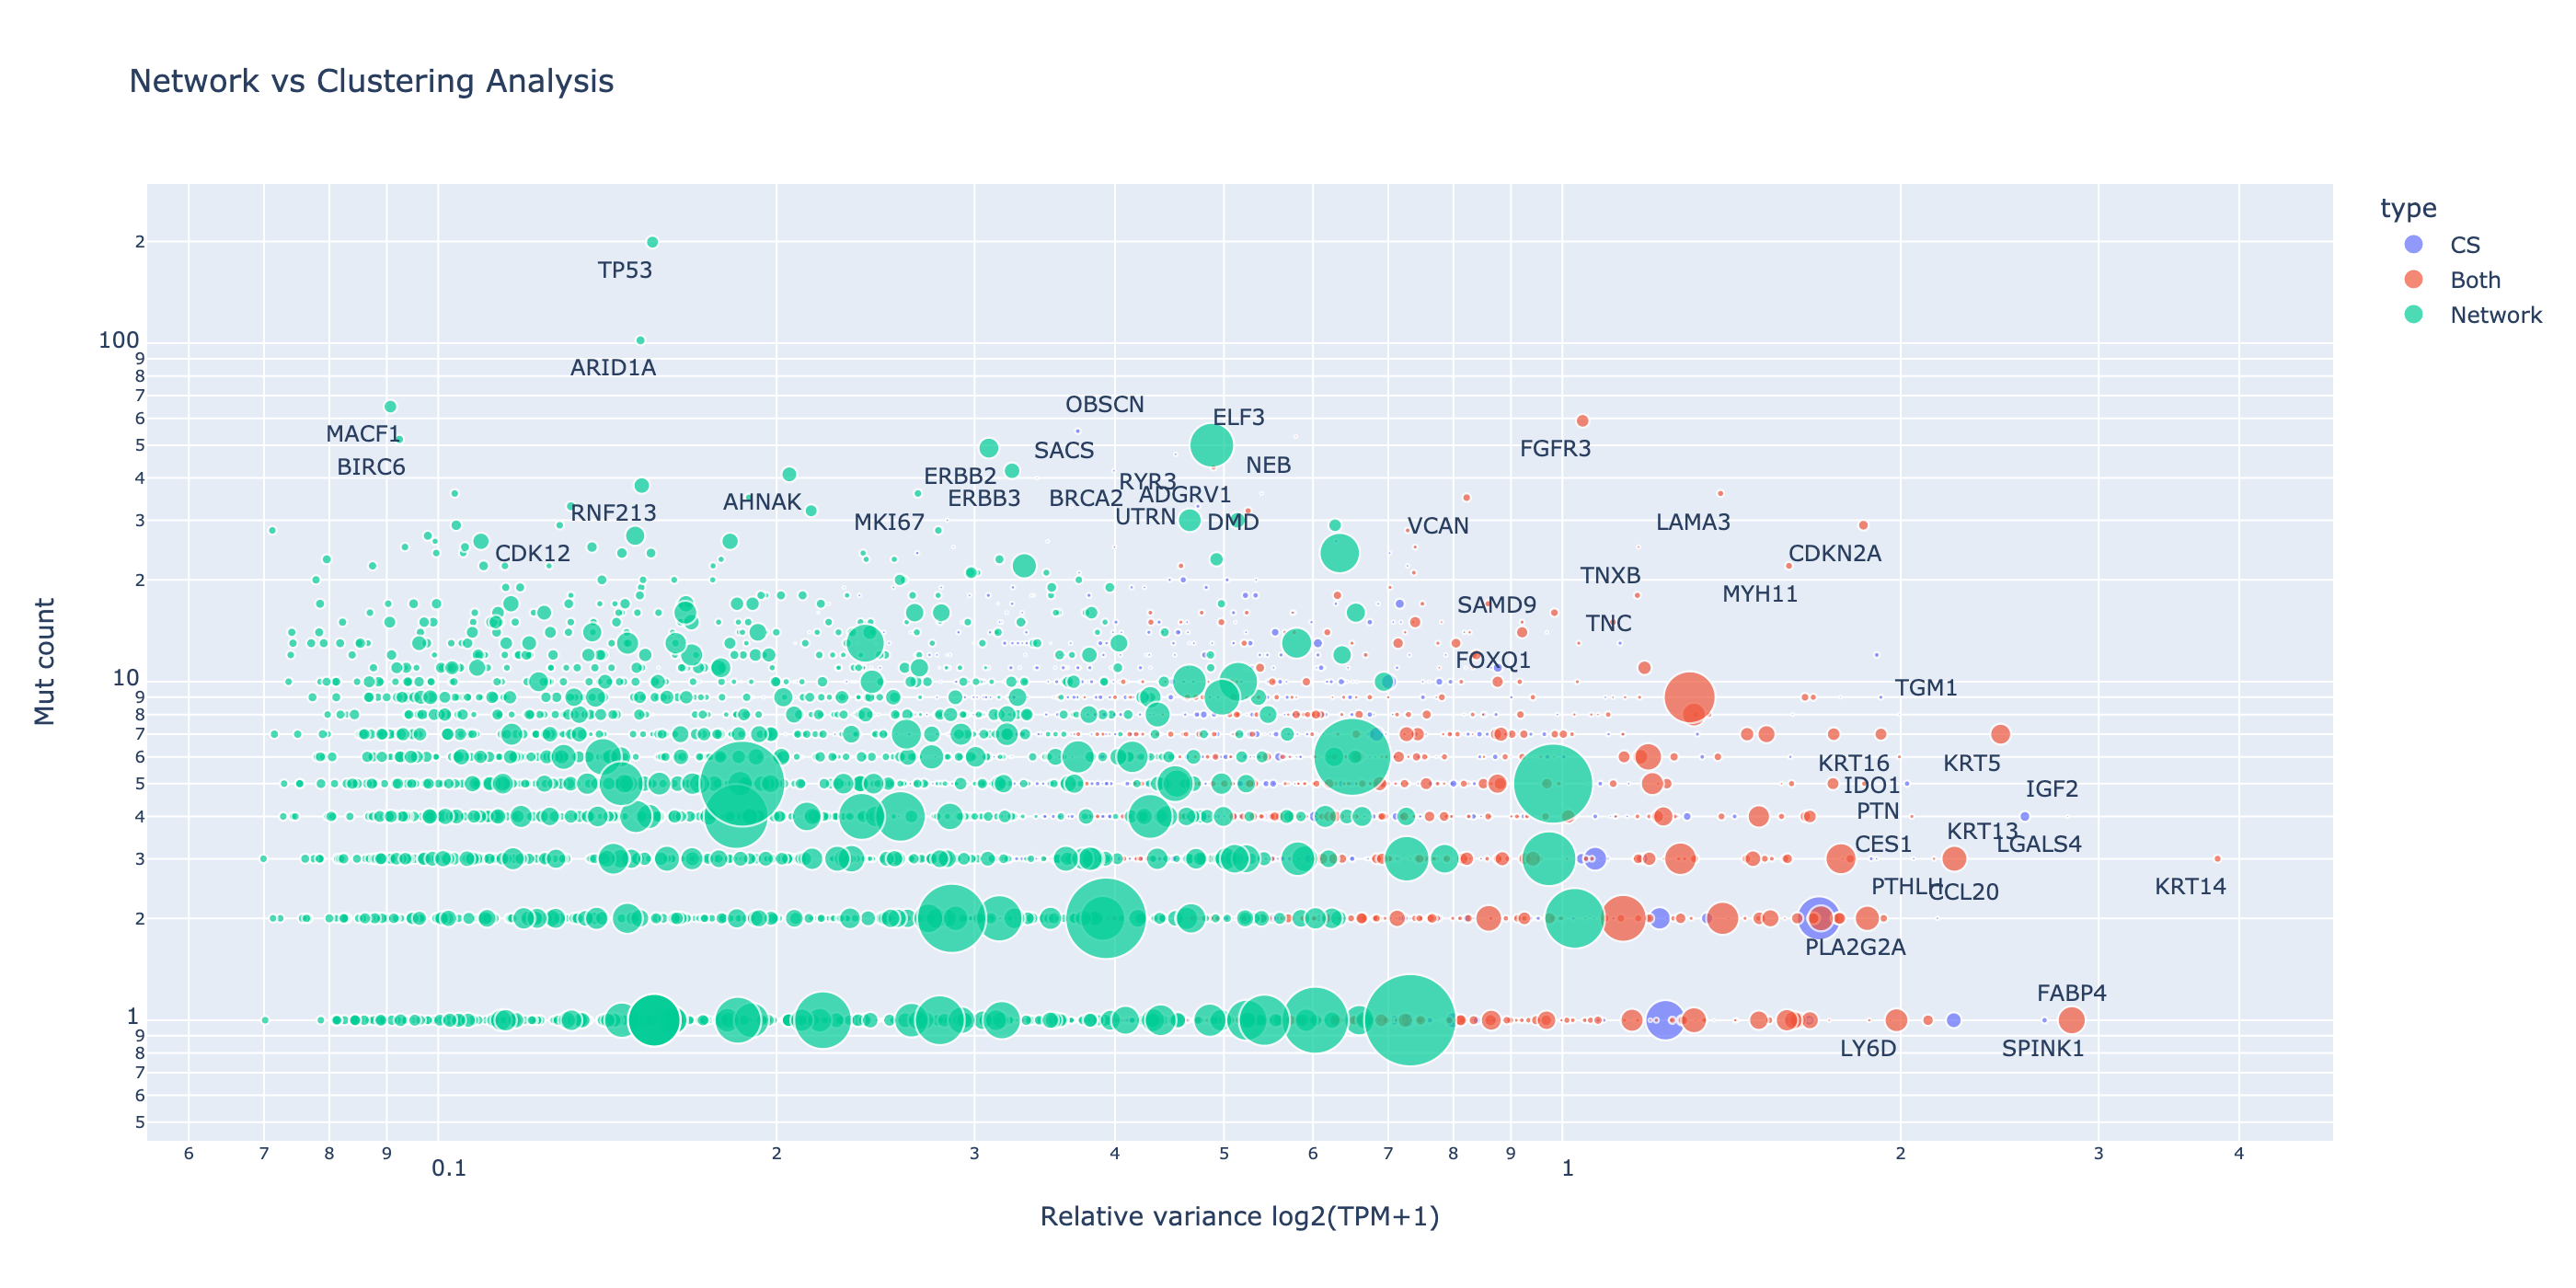
\includegraphics[width=1.0\textwidth,height=0.7\textheight,keepaspectratio]{Sections/Network_I/Resources/Tum_network/ClusteringAnalysis_vs_Network_3.png}
    \caption{Network selection vs. Clustering Analysis. Blue points are represented by the genes selected exclusively by the highest median standard deviation ratio, the green by the network and red by both approaches. The size of the points is the median expression of the genes in TCGA. To avoid log values of 0 the mutations count were offset by one.}
    \label{fig:N_I:network_ca_selection}
\end{figure}


The $\approx2.8K$ genes selected through the network are compared with the 3K most relative varied. Between the two sets of genes there are 1733 different genes and 746 shared. In Figure \ref{fig:N_I:network_ca_selection} the two sets of genes are plotted against the Mutation Burden across the TCGA cohort (Y-axis) and the relative variance across (X-axis). Blue points are represented by the genes selected exclusively by the highest median standard deviation ratio, the green by the network and red by both approaches. As expected the genes selected only by relative variance are skewed to the right picking the highly mutated genes that also have a high variance. Contrary, the network approach (using ModCon) not only selects most of the varied genes but also some of the highest mutated genes despite having low variance. The points' size is relative to the median expression in the TCGA cohort and from the Figure \ref{fig:N_I:network_ca_selection} it can be seen that the canonical gene selection does not include the highly expressed genes as the network does.

This comparison shows the power of the network approach which selects not only the highly varied genes but also the ones that have consistent expression values and high mutation burden.

\subsubsection{Conclusion}

The two set of experiments performed in this Section suggest the potential of a network approach to stratify the MIBC. In the first part (Section \ref{s:N_I:weights}), three networks with different weight modifiers were created and analysed. From the network and community detection metrics (see Figure \ref{fig:N_I:net_metrics_tum} and Figure\ref{fig:N_I:tum_leiden_modifiers}) we could see that there three networks (Standard, Reward and Penalised) perform similarly but, importantly, exhibit different MIBC subgroups from the canonical methods. Based on this, we explored the differences in the selected genes from the Clustering Analysis and the network approach (depicted in Figure \ref{fig:N_I:network_ca_selection}) which showed that the network is capable to pick genes with a wider a range of properties. Genes with higher mutation, magnitude and the highest variance are selected by our network approach, while the standard approach selects only with the highest relative variance.

Both experiments show the advantages of the network approach in finding new potential cancer subgroups. However, the data integration strategy in this section does not exhibit the desired results.

% \newpage

% \subsubsection{Checkpoint}:
% \begin{todolist}
%     \item [\done] Describe weight modifiers and the motivation behind them
%     \item [\done] Describe how ModCon was adapted and Spearman Correlation process 
%     \item [\done] Network stats - between the 3 different types of modifiers. What shall we do?
%     \item [\done] Looking at the mutation representation 
%     \item [\done] Leiden Community detection
%     \item [\done] Sankey comparison
%     \item [\done] Community comparison 
%     \item [\done] Justify the network configurations
%     \item [\done] Discussion and Conclusion
%     \item Survival plots
%     \item Network on gephi? (optional)
%     \item Comparing with Lund? (optional)
%     \item Community analysis (optional). How are the mutated genes represented per community, per TF and per median GE.
% \end{todolist}